\documentclass[10pt,aspectratio=169]{beamer}
\usetheme{Frankfurt}
\usecolortheme{beaver}
\definecolor{darkgreen}{RGB}{0,115,60}
\setbeamercolor{alerted text}{fg=darkgreen!80!gray}
\setbeamercolor*{palette primary}{fg=darkgreen!60!black,bg=gray!30!white}
\setbeamercolor*{palette secondary}{fg=darkgreen!70!black,bg=gray!15!white}
\setbeamercolor*{palette tertiary}{bg=darkgreen!80!black,fg=gray!10!white}
\setbeamercolor*{palette quaternary}{fg=darkgreen,bg=gray!5!white}
\setbeamercolor{titlelike}{parent=palette primary,fg=darkgreen}
\setbeamercolor{block title alerted}{fg=white,bg=darkgreen!80!black}
\setbeamercolor{block body alerted}{bg=darkgreen!8!white}
\setbeamertemplate{navigation symbols}{}
\setbeamertemplate{headline}{}

\usepackage[english,russian]{babel}
\usepackage{fontspec}
\setsansfont{Fira Sans}
\setmonofont{Fira Mono}
\usepackage{tikz}
\usetikzlibrary{calc,positioning,decorations.pathreplacing}
\usepackage{booktabs}
\usepackage{tabularx}
\usepackage{listings}
\usepackage{url}
\usepackage{hyperref}

\lstset{
  basicstyle=\footnotesize\ttfamily,
  columns=fullflexible,
  keepspaces=true,
  breaklines=true,
  commentstyle=\color{gray}
}
\lstdefinelanguage{dockerbash}{
  language=bash,
  morekeywords={docker},
  comment=[l]{\#}
}
\lstdefinelanguage{dockerfile}{
  morekeywords={FROM,AS,WORKDIR,COPY,RUN,CMD,ENTRYPOINT,EXPOSE,USER,ENV,ARG,HEALTHCHECK},
  sensitive=true,
  comment=[l]{\#},
  morestring=[b]"
}
\lstset{language=dockerbash}

\title{Docker: основные команды}
\author{Селиверстов А., Слесарева Е.}
\institute{Санкт-Петербургский политехнический университет Петра Великого\\
Группа 5040102/60101}
\date{31 октября 2026 г.}

\newcommand{\ulink}[2]{\href{#1}{\textcolor{blue!60!black}{\underline{#2}}}}
\newcommand{\doclink}[2]{\href{#1}{\textcolor{blue!60!black}{#2}}}
\def\figsline{}
\def\docsline{}
\newcommand{\figs}[1]{\gdef\figsline{#1\par}}
\newcommand{\docs}[1]{\gdef\docsline{Документация: #1}}
\setbeamertemplate{footline}{%
  \hbox to \paperwidth{%
    \hspace*{3pt}%
    \raisebox{0pt}[0pt][0pt]{\parbox[b]{0.88\paperwidth}{\raggedright\tiny\figsline\docsline}}%
    \hfill
    \raisebox{0pt}[\height][0pt]{\usebeamerfont{page number in head/foot}\usebeamercolor[fg]{page number in head/foot}\insertframenumber{} / \inserttotalframenumber}%
    \hspace*{2ex}}%
  \vskip5pt
  \global\let\figsline\empty
  \global\let\docsline\empty}


% схема VM vs контейнеры (по мотивам Docker vs VM, Drinkler, CC BY-SA 4.0)
\definecolor{lyY}{HTML}{F8E6C4}\definecolor{lyG}{HTML}{DCEBD5}\definecolor{lyR}{HTML}{F1D0D0}
\definecolor{lyHW}{HTML}{C9DAF8}\definecolor{lyOS}{HTML}{D9D9D9}\definecolor{lyHV}{HTML}{F2F2F2}\definecolor{lyDE}{HTML}{E6EDF8}
\newcommand{\lybox}[7]{% x y w h цвет текст шрифт
  \draw[line width=0.5pt, fill=#5] (#1,#2) rectangle ++(#3,#4);
  \node[align=center, font=#7, inner sep=0pt] at ($(#1,#2)+0.5*(#3,#4)$) {#6};}
\newcommand{\lyapps}[1]{%
  \foreach \c/\x/\n in {lyY/0/1,lyG/2.55/2,lyR/5.1/3}{
    \lybox{\x}{#1}{2.3}{0.6}{\c}{Bins/Libs}{\lyS}
    \lybox{\x}{#1+0.75}{2.3}{0.6}{\c}{App \n}{\lyS}}}
\newcommand{\lybase}[2]{%
  \lybox{0}{0}{7.4}{1.2}{lyHW}{Hardware}{\lyL}
  \lybox{0}{1.35}{7.4}{0.85}{lyOS}{#1}{\lyS}}
\newcommand{\lyS}{\fontsize{4.6pt}{5pt}\selectfont}\newcommand{\lyL}{\scriptsize}
\newcommand{\vmstack}[1][0.33cm]{\begin{tikzpicture}[x=#1,y=#1]
  \lybase{Host Operating System}{}
  \lybox{0}{2.35}{7.4}{0.85}{lyHV}{Hypervisor}{\lyL}
  \foreach \c/\x in {lyY/0,lyG/2.55,lyR/5.1}{\lybox{\x}{3.35}{2.3}{1.9}{\c}{Guest\\OS}{\lyL}}
  \lyapps{5.4}
  \node[font=\lyL] at (3.7,-0.6) {Virtual Machines};
\end{tikzpicture}}
\newcommand{\ctstack}[1][0.33cm]{\begin{tikzpicture}[x=#1,y=#1]
  \lybase{Operating System}{}
  \lybox{0}{2.35}{7.4}{0.85}{lyDE}{Docker Engine}{\lyL}
  \lyapps{3.35}
  \path (0,6.7);
  \node[font=\lyL] at (3.7,-0.6) {Containers};
\end{tikzpicture}}

\begin{document}

\maketitle

\section{Что такое Docker}

\begin{frame}{Введение в Docker: works well for me!}
  \begin{columns}[c]
    \begin{column}{0.36\textwidth}
      \centering
      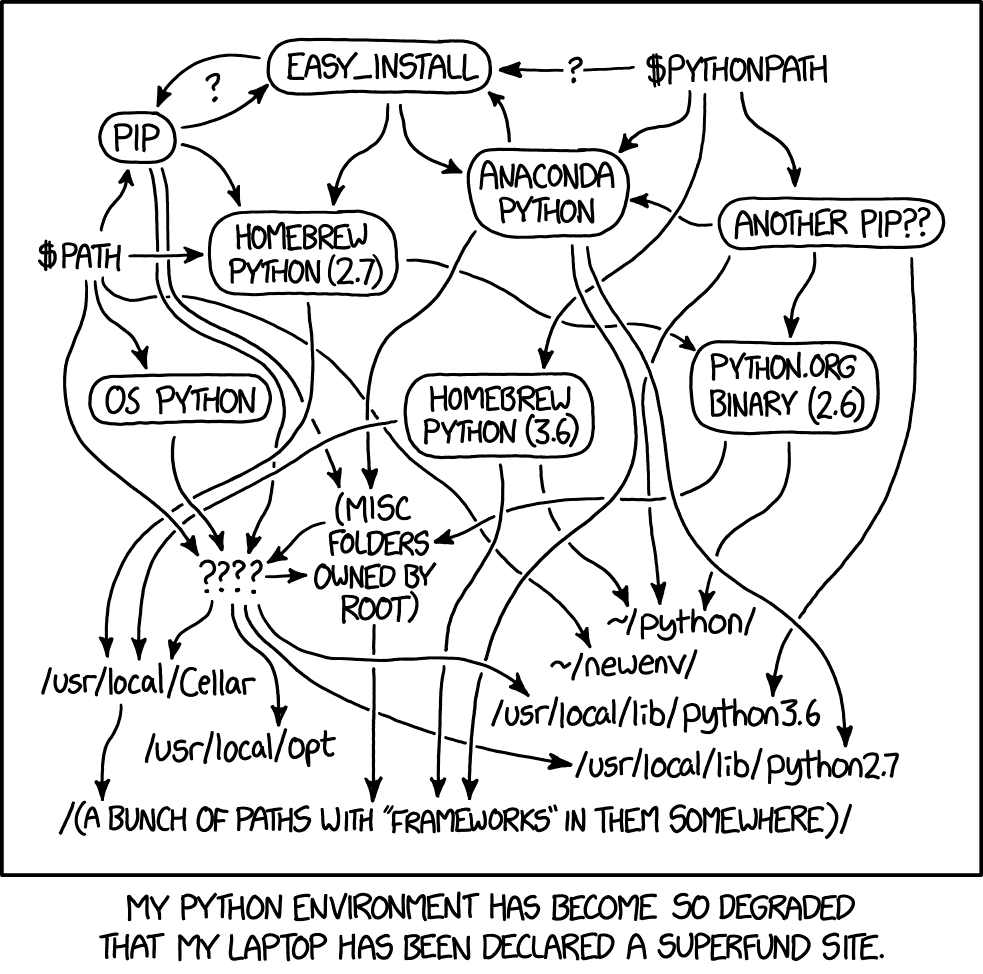
\includegraphics[width=\linewidth]{img/xkcd-python-environment.png}
    \end{column}
    \begin{column}{0.24\textwidth}
      \centering
      \ctstack[0.42cm]
    \end{column}
    \begin{column}{0.36\textwidth}
      \small
      Docker упаковывает программу вместе с окружением в образ и запускает её в контейнере: изолированном процессе на общем ядре ОС.
    \end{column}
  \end{columns}

  \medskip
  \centering
  \scriptsize
  \renewcommand{\arraystretch}{1.2}
  \begin{tabular}{|>{\raggedright\arraybackslash}p{0.15\textwidth}|>{\raggedright\arraybackslash}p{0.75\textwidth}|}
    \hline
    \textbf{ОС} & \textbf{Где работает контейнер} \\ \hline
    Linux & прямо на ядре хоста как обычный процесс. Docker Engine изолирует его (namespaces) и ограничивает ресурсы (cgroups) \\ \hline
    macOS & в Linux-ВМ, которую поднимает Docker Desktop \\ \hline
    Windows & в Linux-ВМ, обычно через WSL~2 \\ \hline
    Другой процессор & образ amd64 на arm64 (Mac с Apple): команды эмулируются, это медленнее \\ \hline
  \end{tabular}
  \figs{Рисунки: \doclink{https://xkcd.com/1987/}{xkcd 1987}, Randall Munroe, CC BY-NC 2.5; схема по мотивам \doclink{https://commons.wikimedia.org/wiki/File:Dockervsvm.jpg}{Docker vs VM}, Drinkler, CC BY-SA 4.0.}
  \docs{\doclink{https://docs.docker.com/get-started/docker-overview/}{Docker overview}, \doclink{https://docs.docker.com/engine/security/\#kernel-namespaces}{Engine security}, \doclink{https://docs.docker.com/desktop/features/vmm/}{Docker Desktop VMM}}
\end{frame}

\begin{frame}{Контейнер vs VM}
  \begin{columns}[c]
    \begin{column}{0.49\textwidth}
      \centering
      \vmstack[0.36cm]\hspace{0.25cm}\ctstack[0.36cm]
    \end{column}
    \begin{column}{0.48\textwidth}
      \scriptsize
      \renewcommand{\arraystretch}{1.3}
      \begin{tabular}{|>{\raggedright\arraybackslash}p{0.19\linewidth}|>{\raggedright\arraybackslash}p{0.36\linewidth}|>{\raggedright\arraybackslash}p{0.27\linewidth}|}
        \hline
        & \textbf{Виртуальная машина} & \textbf{Контейнер} \\ \hline
        ОС & своя гостевая ОС со своим ядром & ядро хоста \\ \hline
        Размер образа & десятки ГБ & десятки МБ \\ \hline
        Запуск & медленно: загружается ОС & быстро: один процесс \\ \hline
        Память & гостевая ОС занимает память всегда & только программа \\ \hline
        Процессор & расходы на гипервизор и гостевую ОС & как у обычного процесса \\ \hline
        Изоляция & сильнее: отдельное ядро & слабее: ядро общее \\ \hline
      \end{tabular}
    \end{column}
  \end{columns}
  \figs{Схема по мотивам \doclink{https://commons.wikimedia.org/wiki/File:Dockervsvm.jpg}{Docker vs VM}, Drinkler, CC BY-SA 4.0, Wikimedia Commons.}
  \docs{\doclink{https://www.docker.com/resources/what-container/}{docker.com: What is a container?}}
\end{frame}

\section{Введение}

\begin{frame}{Введение}
  \centering
  \begin{tikzpicture}[
      box/.style={draw, rounded corners, minimum width=2.6cm, minimum height=0.75cm, align=center, fill=gray!12},
      pic/.style={inner sep=0pt},
      >=latex
    ]
    \foreach \x/\f/\t in {-4.65/archive.jpg/Реестр (registry), 0/blueprint.png/Образ (image), 4.65/house.jpg/Контейнер (container)} {
      \node[pic] at (\x,1.75) {\includegraphics[width=4.2cm,height=2.6cm,keepaspectratio]{img/\f}};
      \node[font=\bfseries] at (\x,3.45) {\t};
    }
    \node[box] (registry) at (-4.65,-0.35) {Docker Hub\\\footnotesize реестр образов};
    \node[box] (image) at (0,-0.35) {Образ\\(image)};
    \node[box] (container) at (4.65,-0.35) {Контейнер\\(container)};
    \node[box] (dockerfile) at (0,-2.0) {Dockerfile\\\footnotesize рецепт сборки};

    \draw[->] (dockerfile) -- node[right]{\footnotesize build} (image);
    \draw[->] (image) -- node[above]{\footnotesize run} (container);
    \draw[->] ([yshift=2mm]image.west) -- node[above]{\footnotesize push} ([yshift=2mm]registry.east);
    \draw[->] ([yshift=-2mm]registry.east) -- node[below]{\footnotesize pull} ([yshift=-2mm]image.west);
  \end{tikzpicture}
  \vfill
  \figs{Рисунки: \doclink{https://commons.wikimedia.org/wiki/File:Newton_Farmhouse,_Belvidere-Kirkland_Road,_Belvidere,_Boone_County,_IL_HABS_ILL,4-_,1-_(sheet_1_of_1).png}{чертёж}, \doclink{https://commons.wikimedia.org/wiki/File:Historic_American_Buildings_Survey_Joseph_Hill,_Photographer_May_28,_1936_EAST_ELEVATION_FRONT_-_Newton_Farmhouse,_Belvidere-Kirkland_Road,_Belvidere,_Boone_County,_IL_HABS_ILL,4-_,1-1.tif}{фото дома} (Historic American Buildings Survey), \doclink{https://commons.wikimedia.org/wiki/File:Historic_Preservation_of_Architectural_Drawings_(26973316484).jpg}{архив чертежей} (Architect of the Capitol); Wikimedia Commons.}
  \docs{\doclink{https://docs.docker.com/get-started/docker-overview/\#docker-objects}{Docker overview, раздел Docker objects}}
\end{frame}

\begin{frame}{Анатомия команды}
  \centering
  \begin{tikzpicture}[
      part/.style={font=\large\ttfamily, inner sep=2pt},
      lab/.style={font=\small, align=center, text width=2.6cm}
    ]
    \node[part] (d) {docker};
    \node[part, right=0.35cm of d] (o) {<объект>};
    \node[part, right=0.35cm of o] (a) {<действие>};
    \node[part, right=0.35cm of a] (f) {[флаги]};
    \node[part, right=0.35cm of f] (g) {[аргументы]};
    \draw[decorate, decoration={brace, mirror, amplitude=4pt}] (o.south west) -- (o.south east) coordinate[midway] (mo);
    \node[lab, below=0.25cm of mo] (lo) {тип объекта:\\ container, image, volume, network};
    \node[lab, below=0.2cm of lo, text=darkgreen, font=\footnotesize, text width=4.2cm] {иногда опускается:\\ \texttt{docker run} =\\ \texttt{docker container run}};
    \draw[decorate, decoration={brace, mirror, amplitude=4pt}] (a.south west) -- (a.south east) coordinate[midway] (ma);
    \node[lab, below=0.25cm of ma] {что сделать:\\ run, ls, rm, logs};
    \draw[decorate, decoration={brace, mirror, amplitude=4pt}] (f.south west) -- (f.south east) coordinate[midway] (mf);
    \node[lab, below=0.25cm of mf] {настройки:\\ \texttt{-d}, \texttt{-p 8080:80}};
  \end{tikzpicture}
  \docs{\doclink{https://docs.docker.com/reference/cli/docker/}{справочник Docker CLI}}
\end{frame}

\begin{frame}{help!!}
  \centering
  \makebox[\textwidth][c]{%
    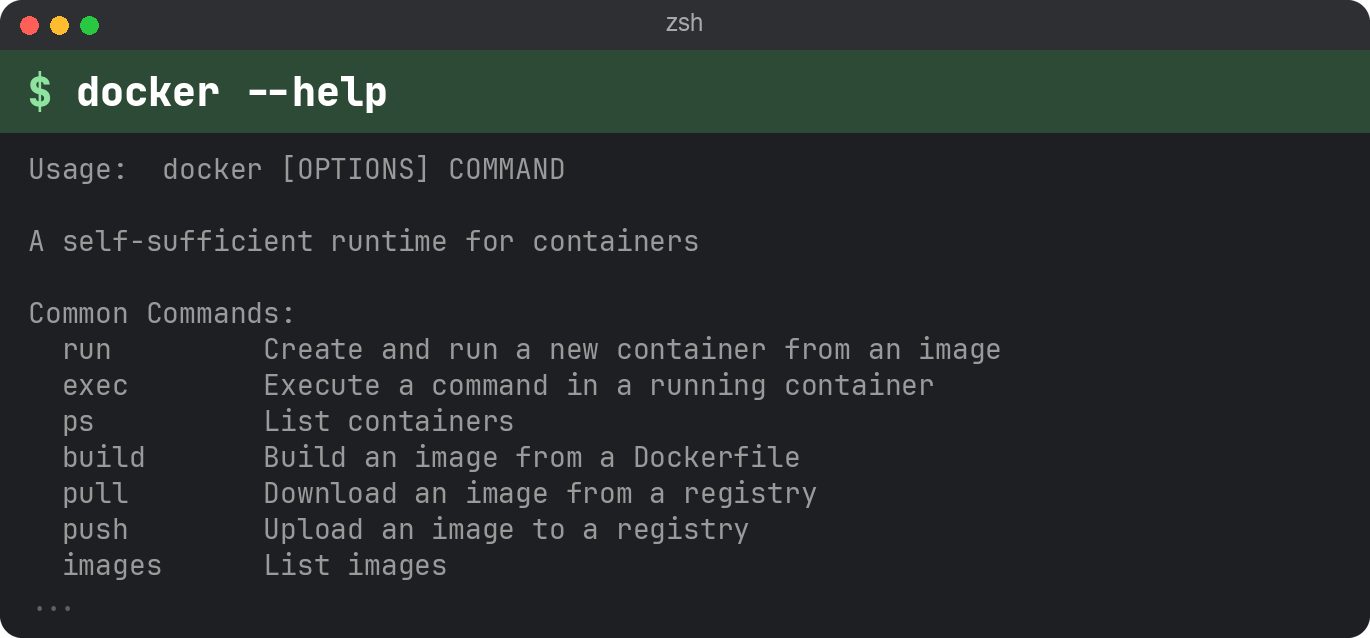
\includegraphics[width=0.465\paperwidth]{img/term/help.png}\hspace{0.015\paperwidth}%
    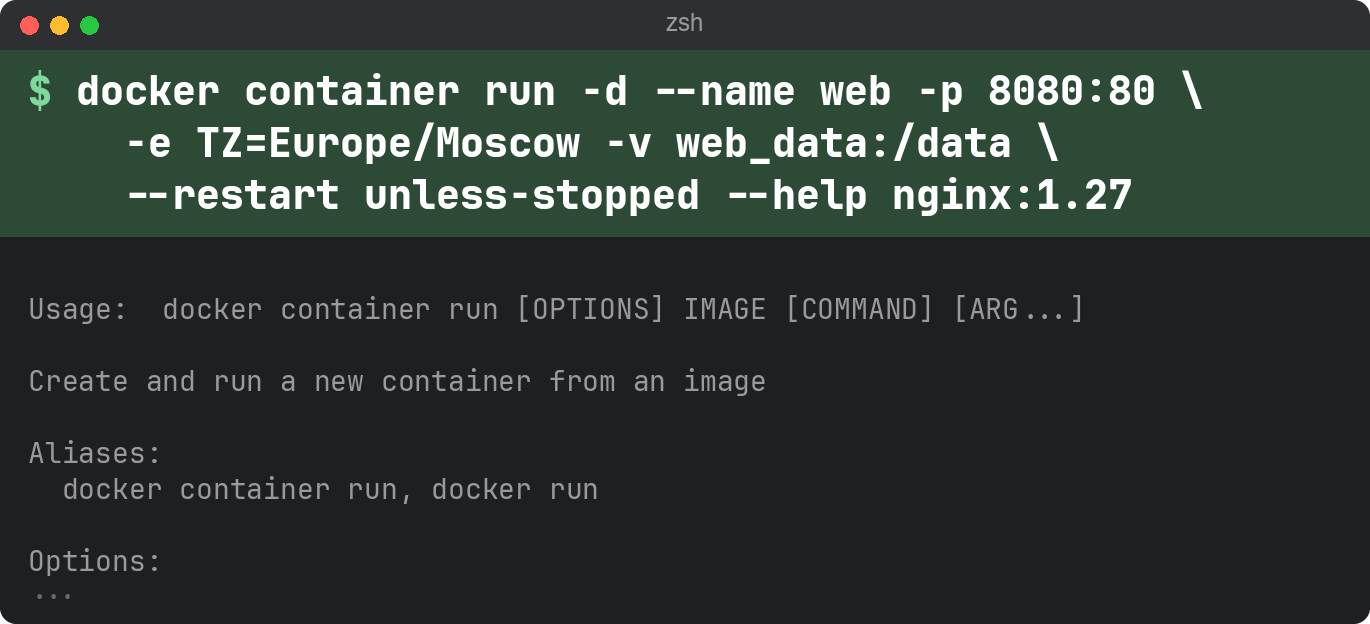
\includegraphics[width=0.465\paperwidth]{img/term/runhelp.png}}\\[0.5em]
  \makebox[\textwidth][c]{%
    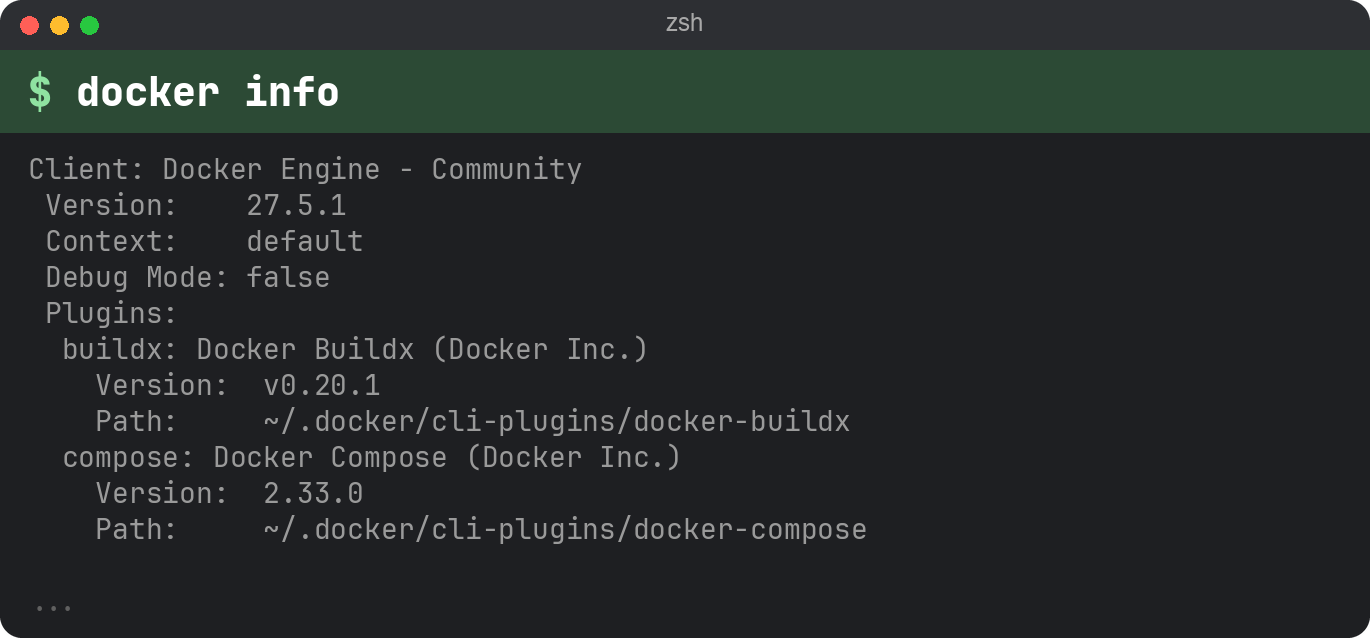
\includegraphics[width=0.465\paperwidth]{img/term/info.png}\hspace{0.015\paperwidth}%
    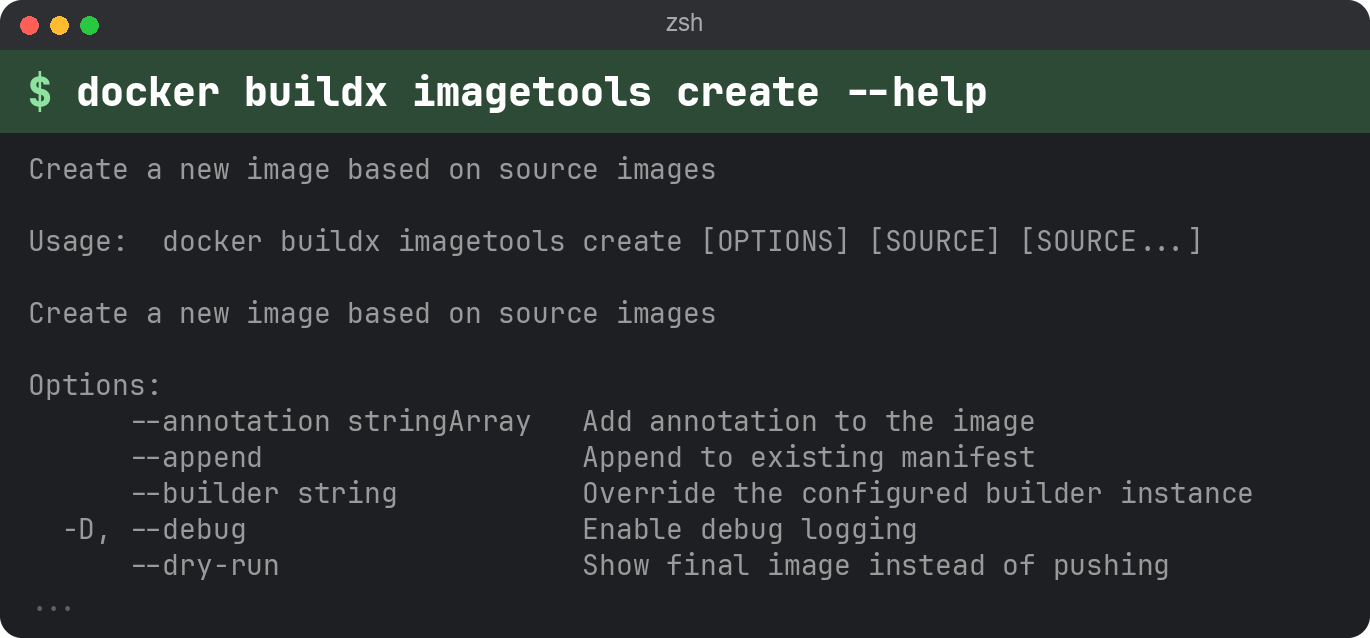
\includegraphics[width=0.465\paperwidth]{img/term/imagetools.png}}
  \docs{\doclink{https://docs.docker.com/reference/cli/docker/}{справочник Docker CLI}, \doclink{https://docs.docker.com/reference/cli/docker/system/info/}{\texttt{docker system info}}}
\end{frame}

\section{Образы}

\begin{frame}
  \centering
  \begin{tikzpicture}[
      box/.style={draw, rounded corners, minimum width=2.6cm, minimum height=0.75cm, align=center, fill=gray!12},
      pic/.style={inner sep=0pt},
      >=latex
    ]
    \foreach \x/\f/\t in {-4.65/archive.jpg/Реестр (registry), 0/blueprint.png/Образ (image), 4.65/house.jpg/Контейнер (container)} {
      \node[pic] at (\x,1.75) {\includegraphics[width=4.2cm,height=2.6cm,keepaspectratio]{img/\f}};
      \node[font=\bfseries] at (\x,3.45) {\t};
    }
    \node[box, fill=darkgreen, draw=darkgreen, text=white, line width=1pt] (registry) at (-4.65,-0.35) {\textbf{Docker Hub}\\\footnotesize реестр образов};
    \node[box] (image) at (0,-0.35) {Образ\\(image)};
    \node[box] (container) at (4.65,-0.35) {Контейнер\\(container)};
    \node[box] (dockerfile) at (0,-2.0) {Dockerfile\\\footnotesize рецепт сборки};

    \draw[->] (dockerfile) -- node[right]{\footnotesize build} (image);
    \draw[->] (image) -- node[above]{\footnotesize run} (container);
    \draw[->, darkgreen, line width=1.4pt] ([yshift=2mm]image.west) -- node[above]{\footnotesize\bfseries push} ([yshift=2mm]registry.east);
    \draw[->, darkgreen, line width=1.4pt] ([yshift=-2mm]registry.east) -- node[below]{\footnotesize\bfseries pull} ([yshift=-2mm]image.west);
  \end{tikzpicture}
  \vfill
  \figs{Рисунки: \doclink{https://commons.wikimedia.org/wiki/File:Newton_Farmhouse,_Belvidere-Kirkland_Road,_Belvidere,_Boone_County,_IL_HABS_ILL,4-_,1-_(sheet_1_of_1).png}{чертёж}, \doclink{https://commons.wikimedia.org/wiki/File:Historic_American_Buildings_Survey_Joseph_Hill,_Photographer_May_28,_1936_EAST_ELEVATION_FRONT_-_Newton_Farmhouse,_Belvidere-Kirkland_Road,_Belvidere,_Boone_County,_IL_HABS_ILL,4-_,1-1.tif}{фото дома} (Historic American Buildings Survey), \doclink{https://commons.wikimedia.org/wiki/File:Historic_Preservation_of_Architectural_Drawings_(26973316484).jpg}{архив чертежей} (Architect of the Capitol); Wikimedia Commons.}
  \docs{\doclink{https://docs.docker.com/get-started/docker-overview/\#docker-objects}{Docker overview, раздел Docker objects}}
\end{frame}

\begin{frame}{Реестр образов}
  \centering
  \makebox[\textwidth][c]{%
    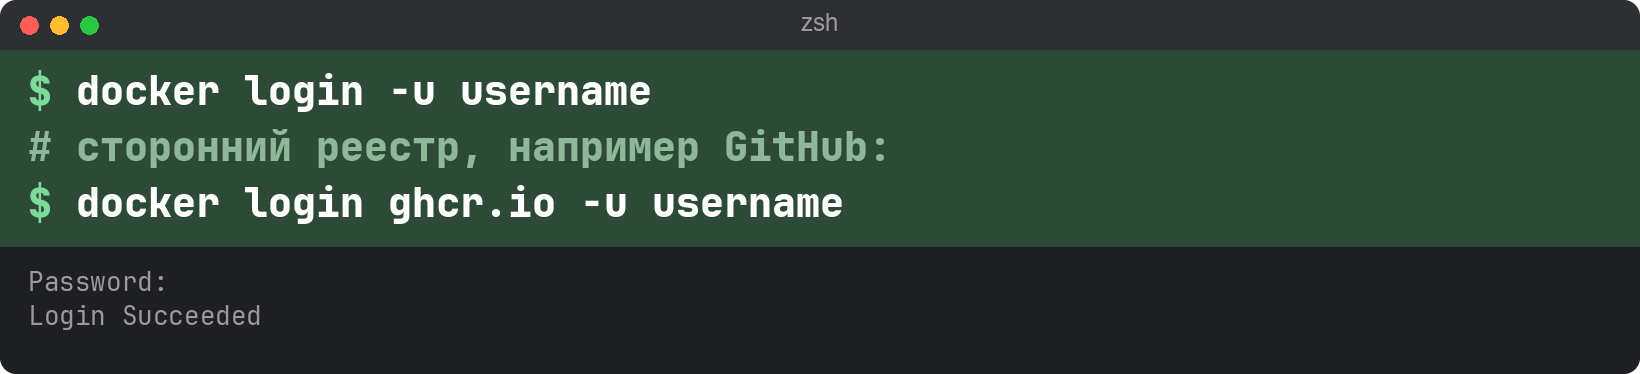
\includegraphics[width=0.47\paperwidth]{img/term/login.png}\hspace{0.015\paperwidth}%
    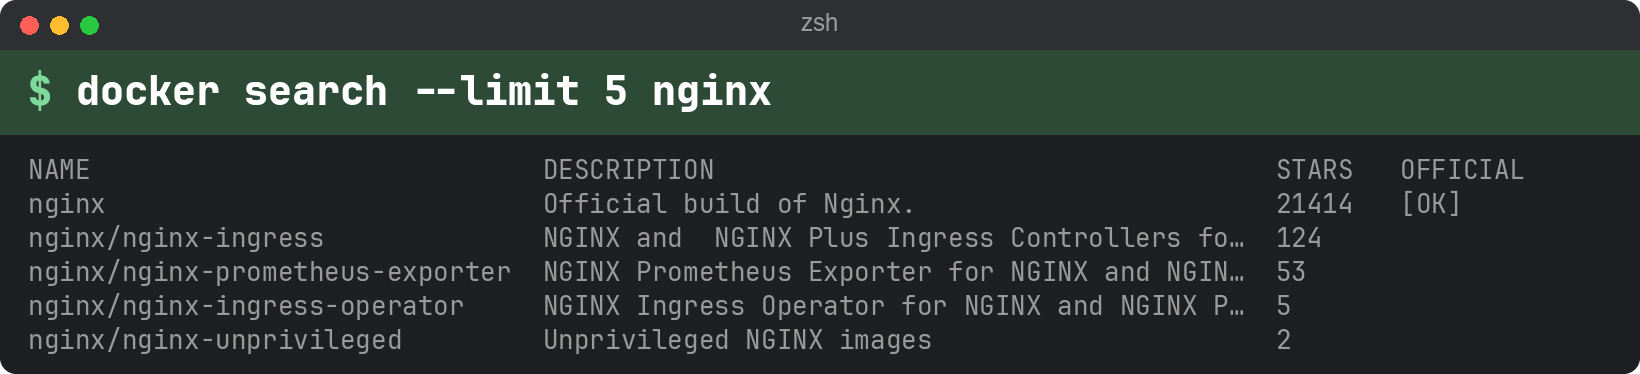
\includegraphics[width=0.47\paperwidth]{img/term/search.png}}\\[0.5em]
  \makebox[\textwidth][c]{%
    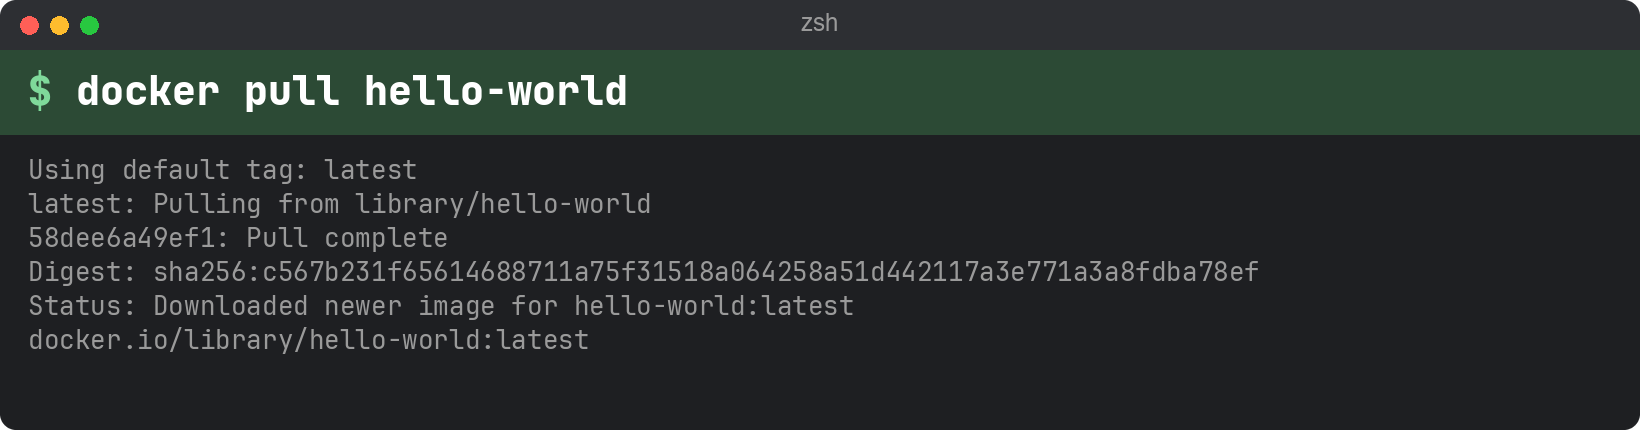
\includegraphics[width=0.47\paperwidth]{img/term/pull.png}\hspace{0.015\paperwidth}%
    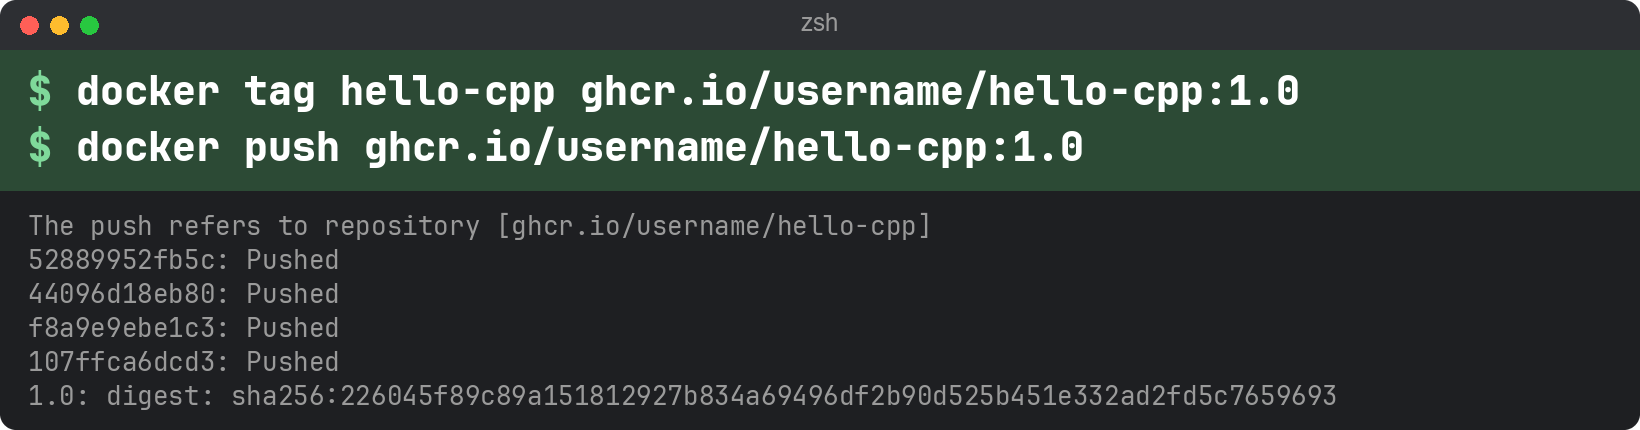
\includegraphics[width=0.47\paperwidth]{img/term/push.png}}
  \docs{\doclink{https://docs.docker.com/get-started/docker-concepts/the-basics/what-is-a-registry/}{What is a registry?}, \doclink{https://docs.github.com/en/packages/working-with-a-github-packages-registry/working-with-the-container-registry}{GitHub Container Registry}}
\end{frame}

\begin{frame}
  \centering
  \begin{tikzpicture}[
      box/.style={draw, rounded corners, minimum width=2.6cm, minimum height=0.75cm, align=center, fill=gray!12},
      pic/.style={inner sep=0pt},
      >=latex
    ]
    \foreach \x/\f/\t in {-4.65/archive.jpg/Реестр (registry), 0/blueprint.png/Образ (image), 4.65/house.jpg/Контейнер (container)} {
      \node[pic] at (\x,1.75) {\includegraphics[width=4.2cm,height=2.6cm,keepaspectratio]{img/\f}};
      \node[font=\bfseries] at (\x,3.45) {\t};
    }
    \node[box, fill=darkgreen!15, draw=darkgreen] (registry) at (-4.65,-0.35) {Docker Hub\\\footnotesize реестр образов};
    \node[box, fill=darkgreen, draw=darkgreen, text=white, line width=1pt] (image) at (0,-0.35) {\textbf{Образ}\\(image)};
    \node[box] (container) at (4.65,-0.35) {Контейнер\\(container)};
    \node[box, fill=darkgreen, draw=darkgreen, text=white, line width=1pt] (dockerfile) at (0,-2.0) {\textbf{Dockerfile}\\\footnotesize рецепт сборки};

    \draw[->, darkgreen, line width=1.4pt] (dockerfile) -- node[right]{\footnotesize\bfseries build} (image);
    \draw[->] (image) -- node[above]{\footnotesize run} (container);
    \draw[->, darkgreen!60] ([yshift=2mm]image.west) -- node[above]{\footnotesize push} ([yshift=2mm]registry.east);
    \draw[->, darkgreen!60] ([yshift=-2mm]registry.east) -- node[below]{\footnotesize pull} ([yshift=-2mm]image.west);
  \end{tikzpicture}
  \vfill
  \figs{Рисунки: \doclink{https://commons.wikimedia.org/wiki/File:Newton_Farmhouse,_Belvidere-Kirkland_Road,_Belvidere,_Boone_County,_IL_HABS_ILL,4-_,1-_(sheet_1_of_1).png}{чертёж}, \doclink{https://commons.wikimedia.org/wiki/File:Historic_American_Buildings_Survey_Joseph_Hill,_Photographer_May_28,_1936_EAST_ELEVATION_FRONT_-_Newton_Farmhouse,_Belvidere-Kirkland_Road,_Belvidere,_Boone_County,_IL_HABS_ILL,4-_,1-1.tif}{фото дома} (Historic American Buildings Survey), \doclink{https://commons.wikimedia.org/wiki/File:Historic_Preservation_of_Architectural_Drawings_(26973316484).jpg}{архив чертежей} (Architect of the Capitol); Wikimedia Commons.}
  \docs{\doclink{https://docs.docker.com/get-started/docker-overview/\#docker-objects}{Docker overview, раздел Docker objects}}
\end{frame}

\begin{frame}{Dockerfile}
  \centering
  \makebox[\textwidth][c]{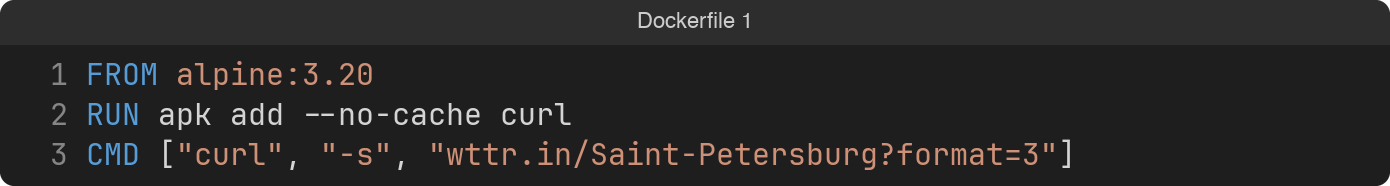
\includegraphics[width=0.84\paperwidth]{img/code/dockerfile1.png}}\\[0.3em]
  \makebox[\textwidth][c]{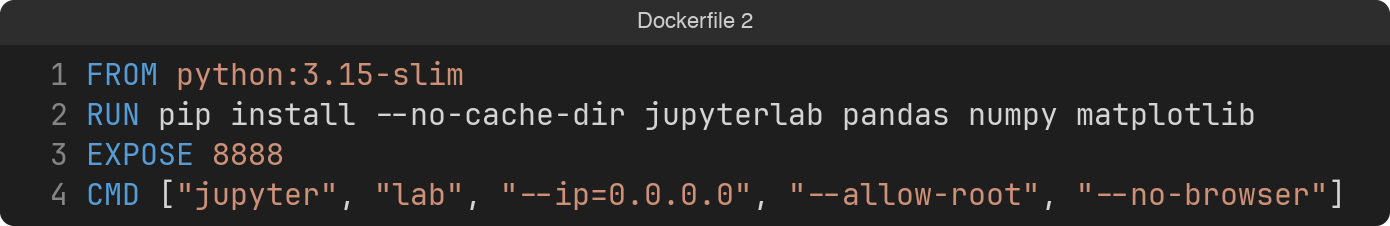
\includegraphics[width=0.84\paperwidth]{img/code/dockerfile2.png}}\\[0.3em]
  \makebox[\textwidth][c]{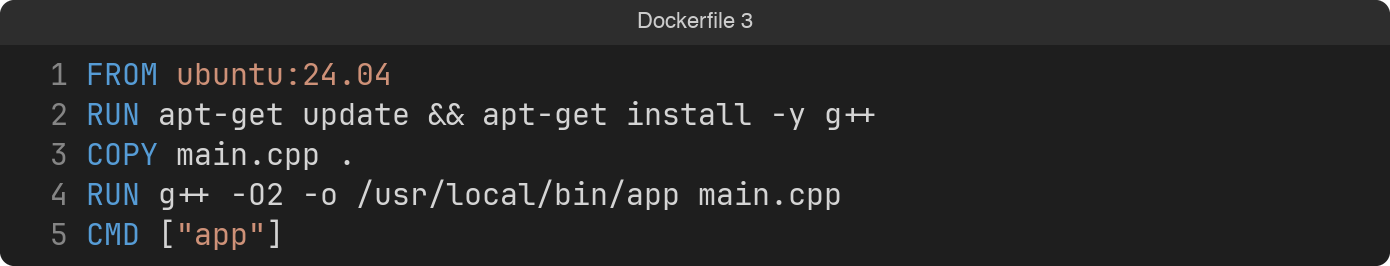
\includegraphics[width=0.84\paperwidth]{img/code/dockerfile3.png}}
  \docs{\doclink{https://docs.docker.com/reference/dockerfile/}{Dockerfile reference}}
\end{frame}

\begin{frame}{Сборка образа}
  \centering
  \makebox[\textwidth][c]{%
    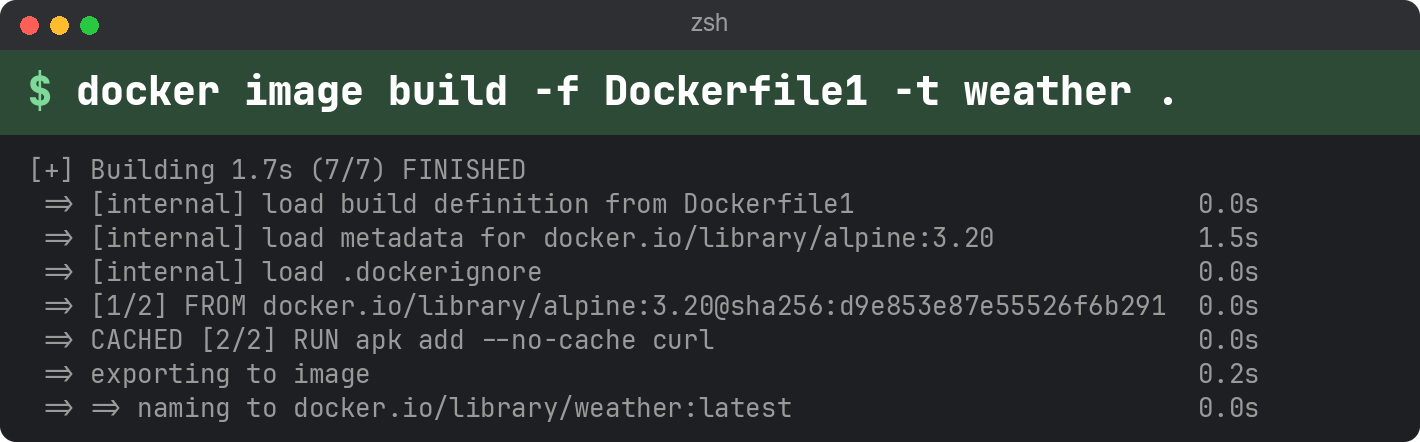
\includegraphics[width=0.465\paperwidth]{img/term/build1.png}\hspace{0.02\paperwidth}%
    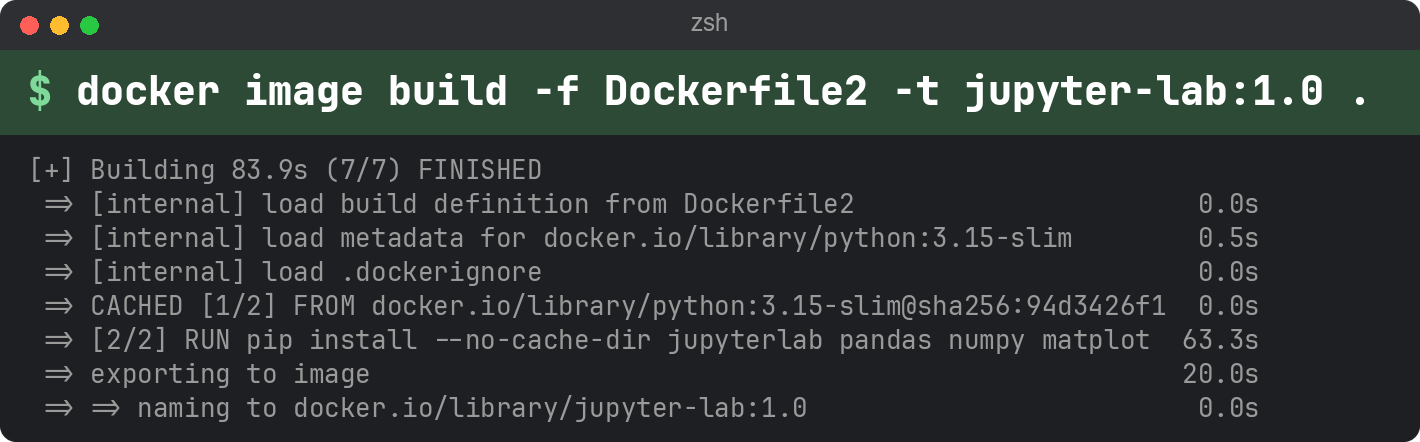
\includegraphics[width=0.465\paperwidth]{img/term/build2.png}}\\[-0.6em]
  \makebox[\textwidth][c]{%
    \raisebox{-\height}{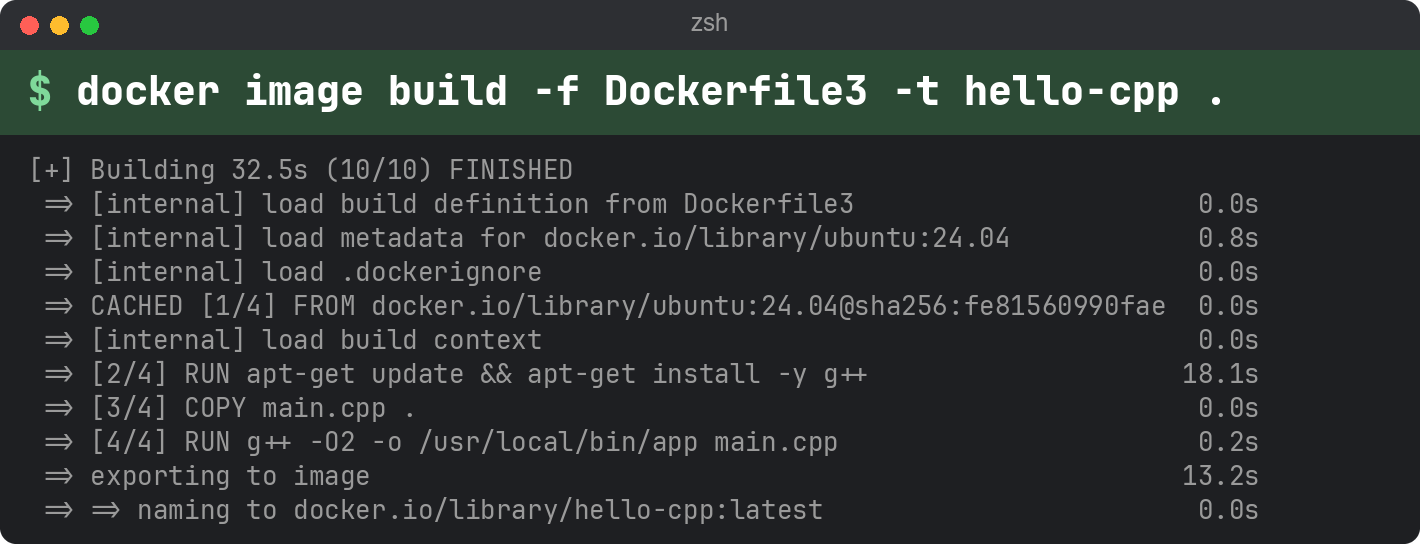
\includegraphics[width=0.465\paperwidth]{img/term/build3.png}}\hspace{0.02\paperwidth}%
    \raisebox{-\height}{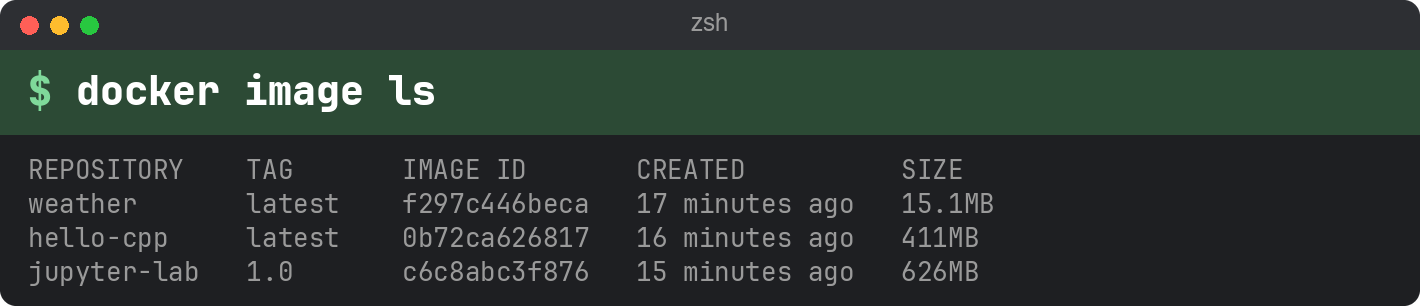
\includegraphics[width=0.465\paperwidth]{img/term/images.png}}}
  \docs{\doclink{https://docs.docker.com/reference/cli/docker/image/build/}{\texttt{docker image build}}, \doclink{https://docs.docker.com/reference/cli/docker/image/ls/}{\texttt{docker image ls}}}
\end{frame}

\begin{frame}{Удаление образов}
  \centering
  \vspace*{\fill}
  \makebox[\textwidth][c]{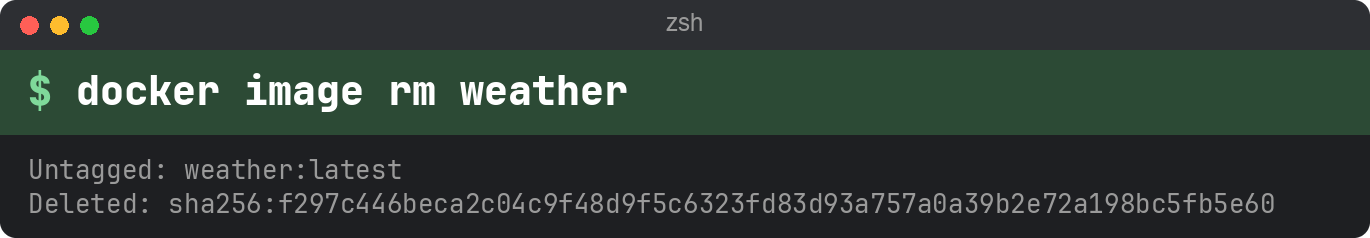
\includegraphics[width=0.7\paperwidth]{img/term/rmi.png}}\\[0.4em]
  \makebox[\textwidth][c]{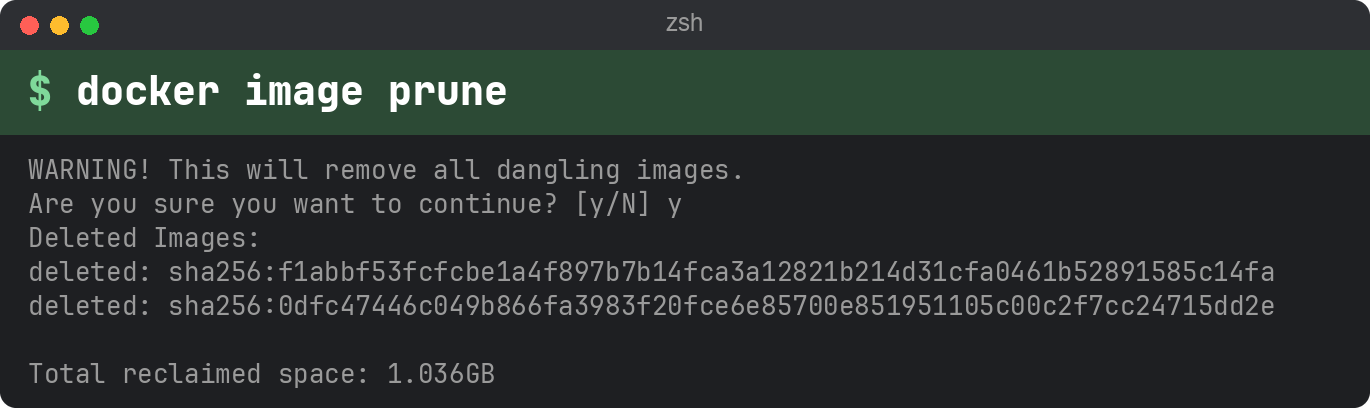
\includegraphics[width=0.7\paperwidth]{img/term/prune.png}}
  \vspace*{\fill}
  \docs{\doclink{https://docs.docker.com/reference/cli/docker/image/rm/}{\texttt{docker image rm}}, \doclink{https://docs.docker.com/reference/cli/docker/image/prune/}{\texttt{docker image prune}}}
\end{frame}

\begin{frame}
  \centering
  \begin{tikzpicture}[
      box/.style={draw, rounded corners, minimum width=2.6cm, minimum height=0.75cm, align=center, fill=gray!12},
      pic/.style={inner sep=0pt},
      >=latex
    ]
    \foreach \x/\f/\t in {-4.65/archive.jpg/Реестр (registry), 0/blueprint.png/Образ (image), 4.65/house.jpg/Контейнер (container)} {
      \node[pic] at (\x,1.75) {\includegraphics[width=4.2cm,height=2.6cm,keepaspectratio]{img/\f}};
      \node[font=\bfseries] at (\x,3.45) {\t};
    }
    \node[box, fill=darkgreen!15, draw=darkgreen] (registry) at (-4.65,-0.35) {Docker Hub\\\footnotesize реестр образов};
    \node[box, fill=darkgreen!15, draw=darkgreen] (image) at (0,-0.35) {Образ\\(image)};
    \node[box, fill=darkgreen, draw=darkgreen, text=white, line width=1pt] (container) at (4.65,-0.35) {\textbf{Контейнер}\\(container)};
    \node[box, fill=darkgreen!15, draw=darkgreen] (dockerfile) at (0,-2.0) {Dockerfile\\\footnotesize рецепт сборки};

    \draw[->, darkgreen!60] (dockerfile) -- node[right]{\footnotesize build} (image);
    \draw[->, darkgreen, line width=1.4pt] (image) -- node[above]{\footnotesize\bfseries run} (container);
    \draw[->, darkgreen!60] ([yshift=2mm]image.west) -- node[above]{\footnotesize push} ([yshift=2mm]registry.east);
    \draw[->, darkgreen!60] ([yshift=-2mm]registry.east) -- node[below]{\footnotesize pull} ([yshift=-2mm]image.west);
  \end{tikzpicture}
  \vfill
  \figs{Рисунки: \doclink{https://commons.wikimedia.org/wiki/File:Newton_Farmhouse,_Belvidere-Kirkland_Road,_Belvidere,_Boone_County,_IL_HABS_ILL,4-_,1-_(sheet_1_of_1).png}{чертёж}, \doclink{https://commons.wikimedia.org/wiki/File:Historic_American_Buildings_Survey_Joseph_Hill,_Photographer_May_28,_1936_EAST_ELEVATION_FRONT_-_Newton_Farmhouse,_Belvidere-Kirkland_Road,_Belvidere,_Boone_County,_IL_HABS_ILL,4-_,1-1.tif}{фото дома} (Historic American Buildings Survey), \doclink{https://commons.wikimedia.org/wiki/File:Historic_Preservation_of_Architectural_Drawings_(26973316484).jpg}{архив чертежей} (Architect of the Capitol); Wikimedia Commons.}
  \docs{\doclink{https://docs.docker.com/get-started/docker-overview/\#docker-objects}{Docker overview, раздел Docker objects}}
\end{frame}

\section{Контейнеры}

\begin{frame}{Запуск контейнера}
  \vspace*{\fill}
  {\centering
  \makebox[\textwidth][c]{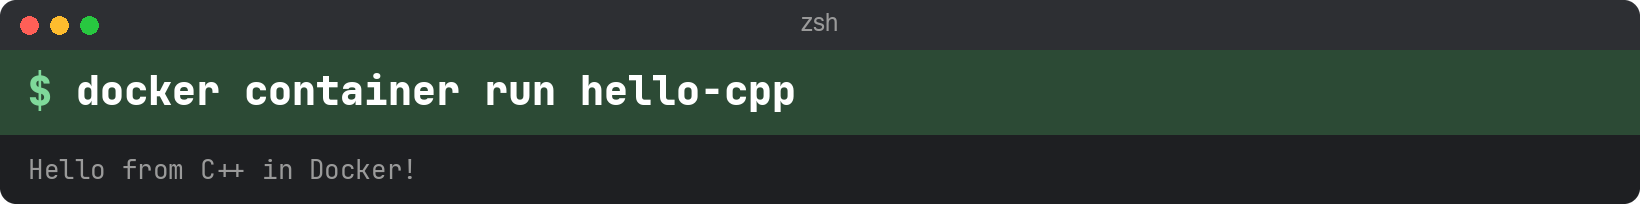
\includegraphics[width=0.7\paperwidth]{img/term/run_hello.png}}\\[0.6em]
  \makebox[\textwidth][c]{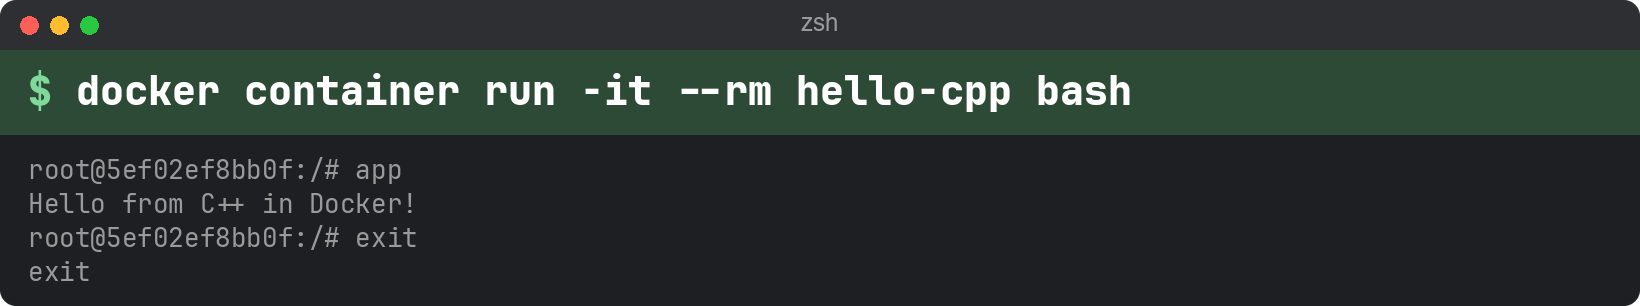
\includegraphics[width=0.7\paperwidth]{img/term/run_it.png}}\par}
  \vspace*{\fill}
  \docs{\doclink{https://docs.docker.com/reference/cli/docker/container/run/}{\texttt{docker container run}}}
\end{frame}

\begin{frame}[fragile]{Запуск контейнера 2}
  \begin{columns}[c]
    \begin{column}{0.66\textwidth}
  Пример из \ulink{https://docs.docker.com/guides/postgresql/}{руководства по PostgreSQL}:
  \begin{lstlisting}
docker container run --rm --name postgres-dev \
  -e POSTGRES_PASSWORD=mysecretpassword \
  -p 5432:5432 \
  -v postgres_data:/var/lib/postgresql \
  -d postgres:18
  \end{lstlisting}
  \vspace{-0.3em}
    \end{column}
    \begin{column}{0.32\textwidth}
    \centering
  \begin{tikzpicture}[
    node distance=0.9cm,
    box/.style={draw, rounded corners, minimum width=2.6cm, minimum height=0.7cm, align=center, fill=gray!12, font=\footnotesize},
    >=latex
  ]
    \node[box] (host) {Хост :5432\\\scriptsize localhost:5432};
    \node[box, below=of host] (cont) {Контейнер :5432};
    \draw[->] (host) -- node[right]{\scriptsize \texttt{-p 5432:5432}} (cont);
  \end{tikzpicture}
    \end{column}
  \end{columns}
  \vspace{0.3em}
  \vspace{-0.5em}

  {\footnotesize
  \renewcommand{\arraystretch}{1.15}
  \begin{tabularx}{\textwidth}{|l|X|}
    \hline
    \textbf{Флаг} & \textbf{Что значит} \\ \hline
    \texttt{-{}-rm} & удалить контейнер, когда он остановится \\ \hline
    \texttt{-{}-name} & задать имя контейнера \\ \hline
    \texttt{-e KEY=value} & задать переменную окружения \\ \hline
    \texttt{-p хост:контейнер} & опубликовать порт контейнера на хосте \\ \hline
    \texttt{-v том:/путь} & подключить том, чтобы данные пережили контейнер \\ \hline
    \texttt{-d} & запустить в фоне \\ \hline
    \texttt{-it} & интерактивная сессия: \texttt{-i} держит STDIN открытым, \texttt{-t} даёт терминал \\ \hline
  \end{tabularx}}
  \vfill
  \docs{\doclink{https://docs.docker.com/reference/cli/docker/container/run/\#publish}{\texttt{-{}-publish}}, \doclink{https://docs.docker.com/reference/cli/docker/container/run/\#env}{\texttt{-{}-env}}, \doclink{https://docs.docker.com/guides/postgresql/}{руководство по PostgreSQL}}
\end{frame}

\begin{frame}{Порядок флагов важен}
  \vspace*{\fill}
  Всё, что стоит после имени образа, Docker не разбирает, а отдаёт внутрь контейнера как команду, которую надо выполнить.

  \vspace{0.8em}

  {\centering\makebox[\textwidth][c]{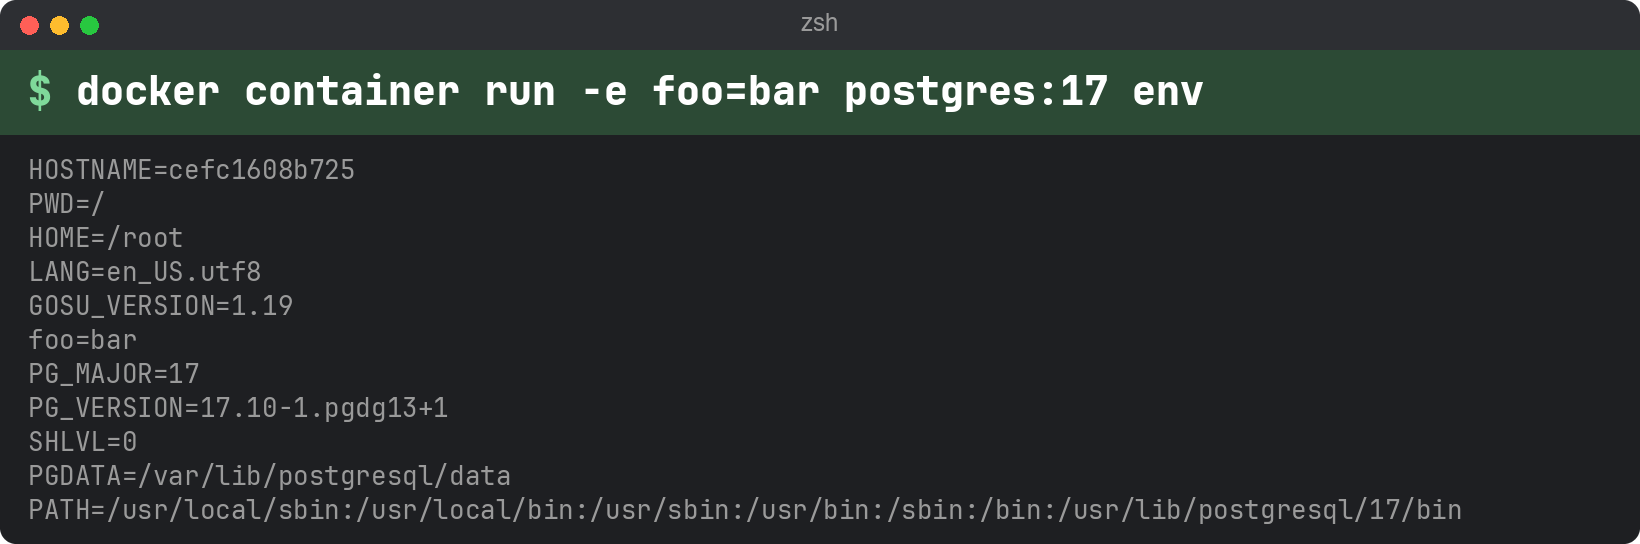
\includegraphics[width=0.55\paperwidth]{img/term/run_env.png}}\par}

  \vspace*{\fill}
  \docs{\doclink{https://docs.docker.com/engine/containers/run/}{Running containers}}
\end{frame}

\begin{frame}{Список контейнеров}
  \vspace*{\fill}
  {\centering\makebox[\textwidth][c]{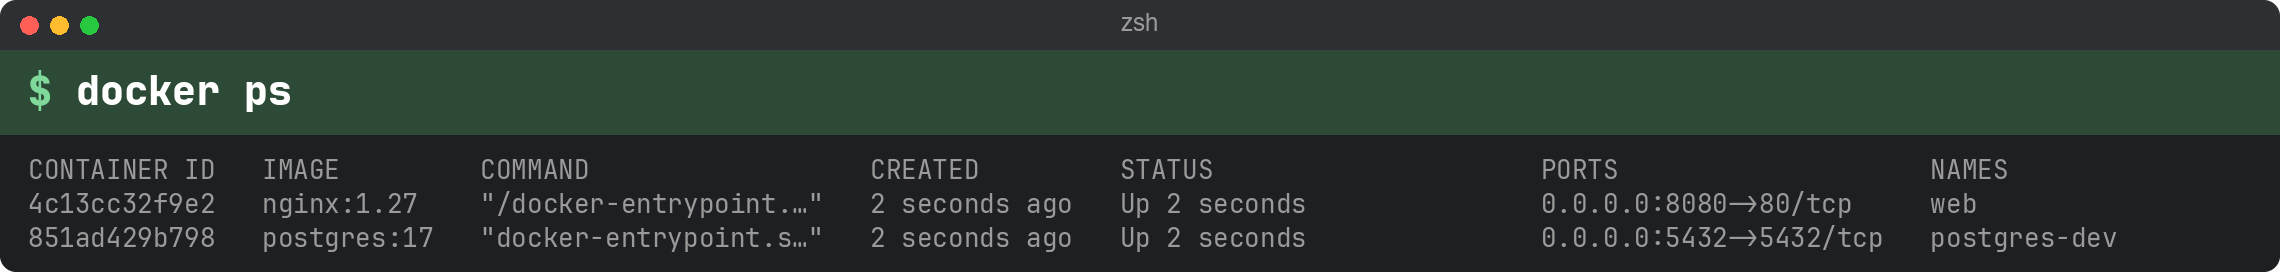
\includegraphics[width=0.84\paperwidth]{img/term/ps.png}}\\[0.3em]
  \makebox[\textwidth][c]{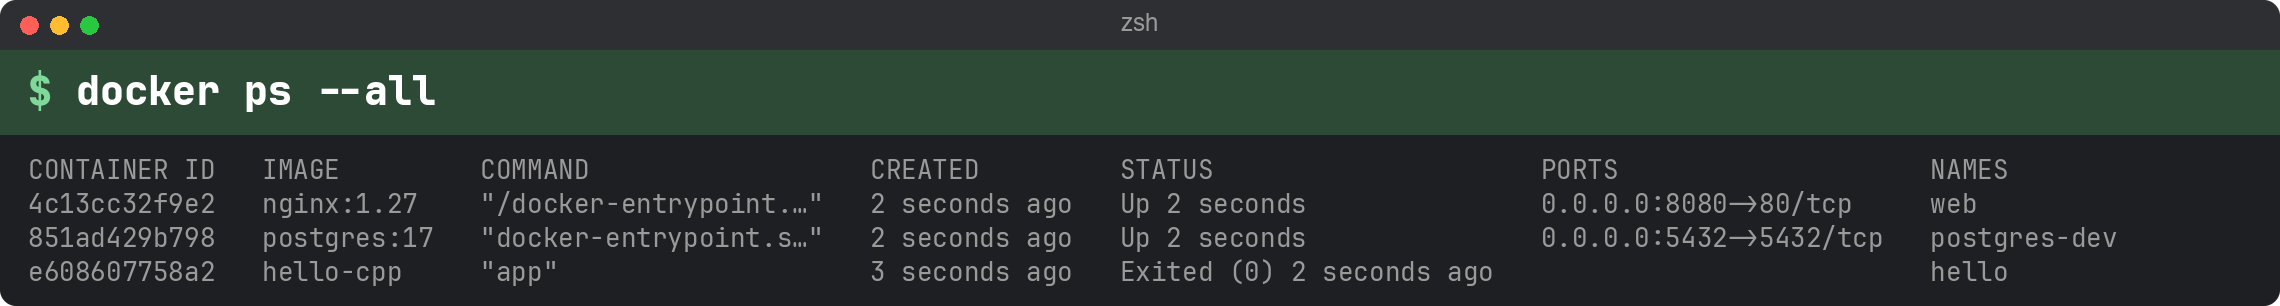
\includegraphics[width=0.84\paperwidth]{img/term/psall.png}}\par}

  
  \vspace*{\fill}
  \docs{\doclink{https://docs.docker.com/reference/cli/docker/container/ls/}{\texttt{docker container ls}}}
\end{frame}

\begin{frame}{Жизненный цикл контейнера}
  \vspace{1.5em}
  {\centering\makebox[\textwidth][c]{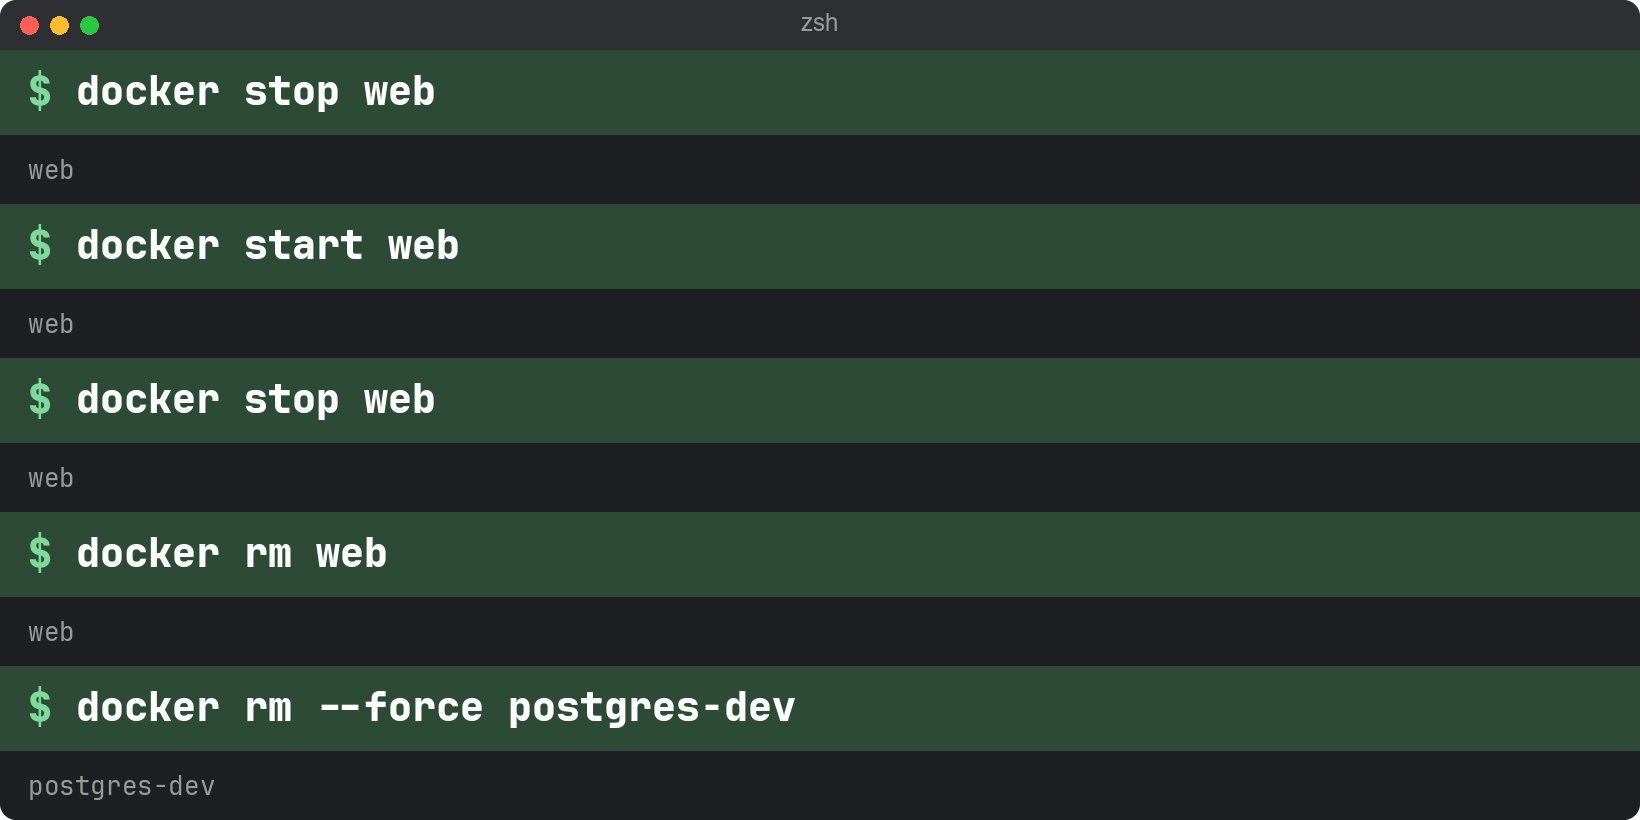
\includegraphics[width=0.42\paperwidth]{img/term/lifecycle.png}}\par}

  \begin{center}
  \begin{tikzpicture}[
    node distance=1.5cm,
    box/.style={draw, rounded corners, minimum width=1.9cm, minimum height=0.8cm, align=center, fill=gray!12, font=\footnotesize, inner sep=3pt},
    >=latex
  ]
    \node[box] (image) {Образ};
    \node[box, right=of image] (up) {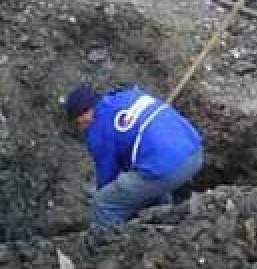
\includegraphics[height=1.3cm]{img/lifecycle/up.png}\\[2pt]Работает\\(Up)};
    \node[box, right=of up] (exited) {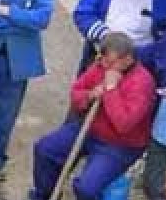
\includegraphics[height=1.3cm]{img/lifecycle/exited.png}\\[2pt]Остановлен\\(Exited)};
    \node[box, right=of exited] (removed) {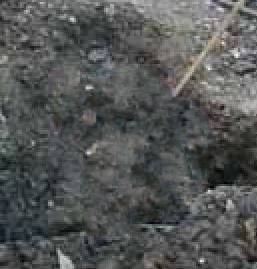
\includegraphics[height=1.3cm]{img/lifecycle/removed.png}\\[2pt]Удалён\\\phantom{(Up)}};

    \draw[->] (image) -- node[above]{\footnotesize run} (up);
    \draw[->] (up) to[bend left=25] node[above]{\footnotesize stop} (exited);
    \draw[->] (exited) to[bend left=25] node[below]{\footnotesize start} (up);
    \draw[->] (exited) -- node[above]{\footnotesize rm} (removed);
  \end{tikzpicture}
  \end{center}
  \vfill
  \figs{Фото: фрагменты снимка с \doclink{http://www.evolo.eu}{evolo.eu} (мем «single worker digging hole»).}
  \docs{\doclink{https://docs.docker.com/reference/cli/docker/container/}{\texttt{docker container}}}
\end{frame}

\begin{frame}{Посмотреть логи}
  \vspace*{\fill}
  {\centering
  \makebox[\textwidth][c]{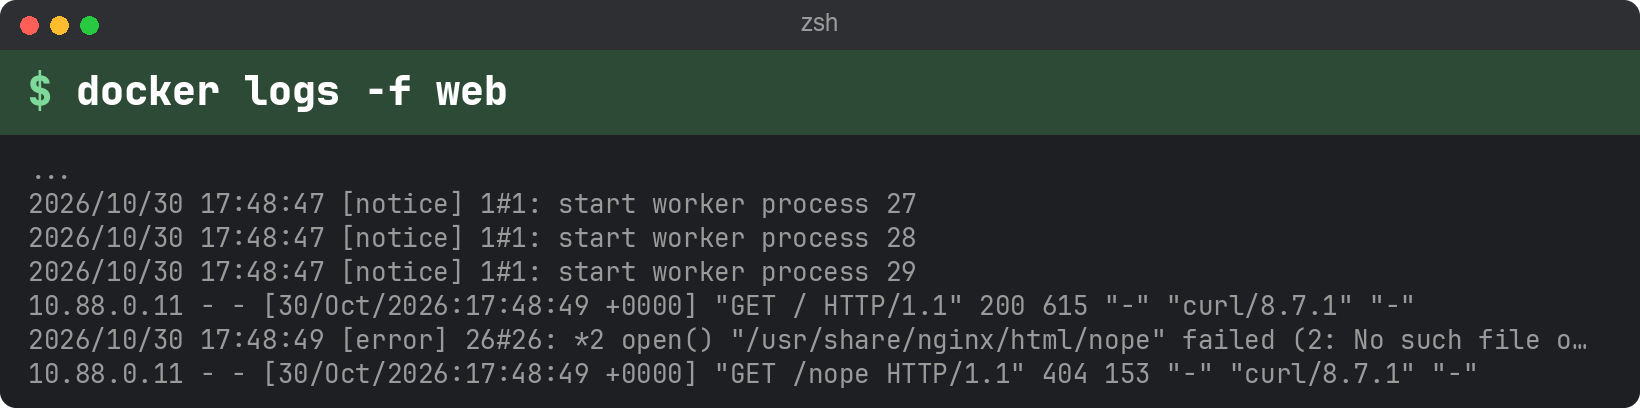
\includegraphics[width=0.7\paperwidth]{img/term/logs.png}}\par}


  \vspace*{\fill}
  \docs{\doclink{https://docs.docker.com/reference/cli/docker/container/logs/}{\texttt{docker container logs}}}
\end{frame}

\section{Обслуживание}

\begin{frame}{Уборка}
  \vspace*{\fill}
  {\centering
  \makebox[\textwidth][c]{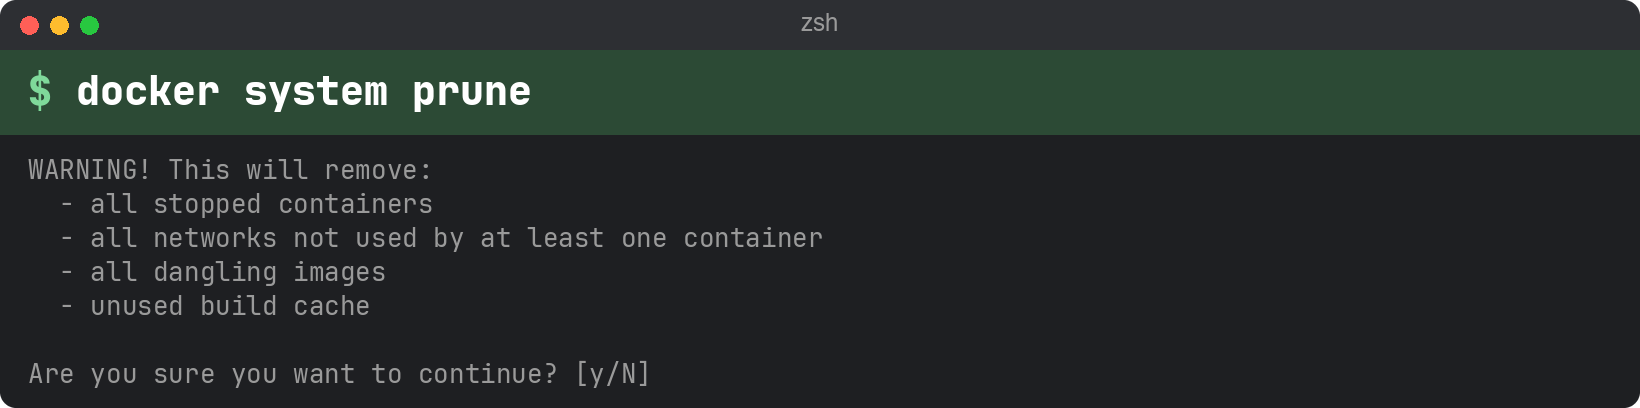
\includegraphics[width=0.6\paperwidth]{img/term/sysprune.png}}\\[0.4em]
  \makebox[\textwidth][c]{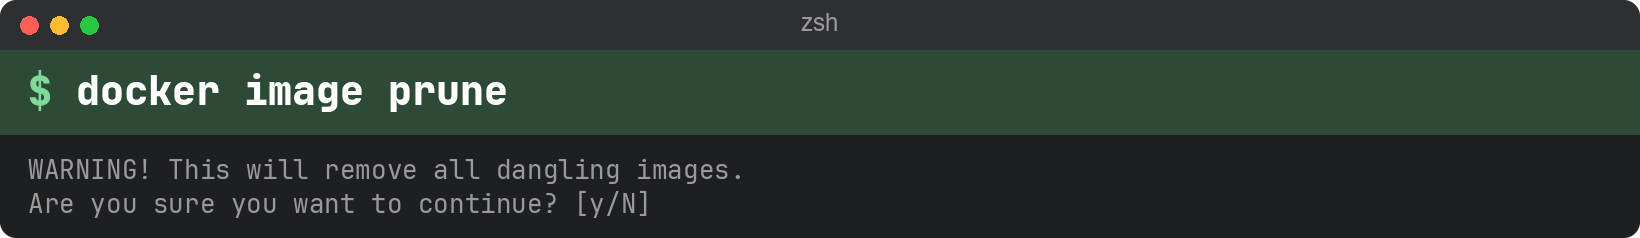
\includegraphics[width=0.6\paperwidth]{img/term/imgprune.png}}\par}


  \vspace*{\fill}
  \docs{\doclink{https://docs.docker.com/reference/cli/docker/system/prune/}{\texttt{docker system prune}}}
\end{frame}

\section{Практика}

\begin{frame}{Всё вместе}
  Сценарий из официального учебника \ulink{https://docs.docker.com/get-started/tutorials/run-an-app/}{Get started: Run an app}. Посередине добавлены команды проверки.

  {\centering\makebox[\textwidth][c]{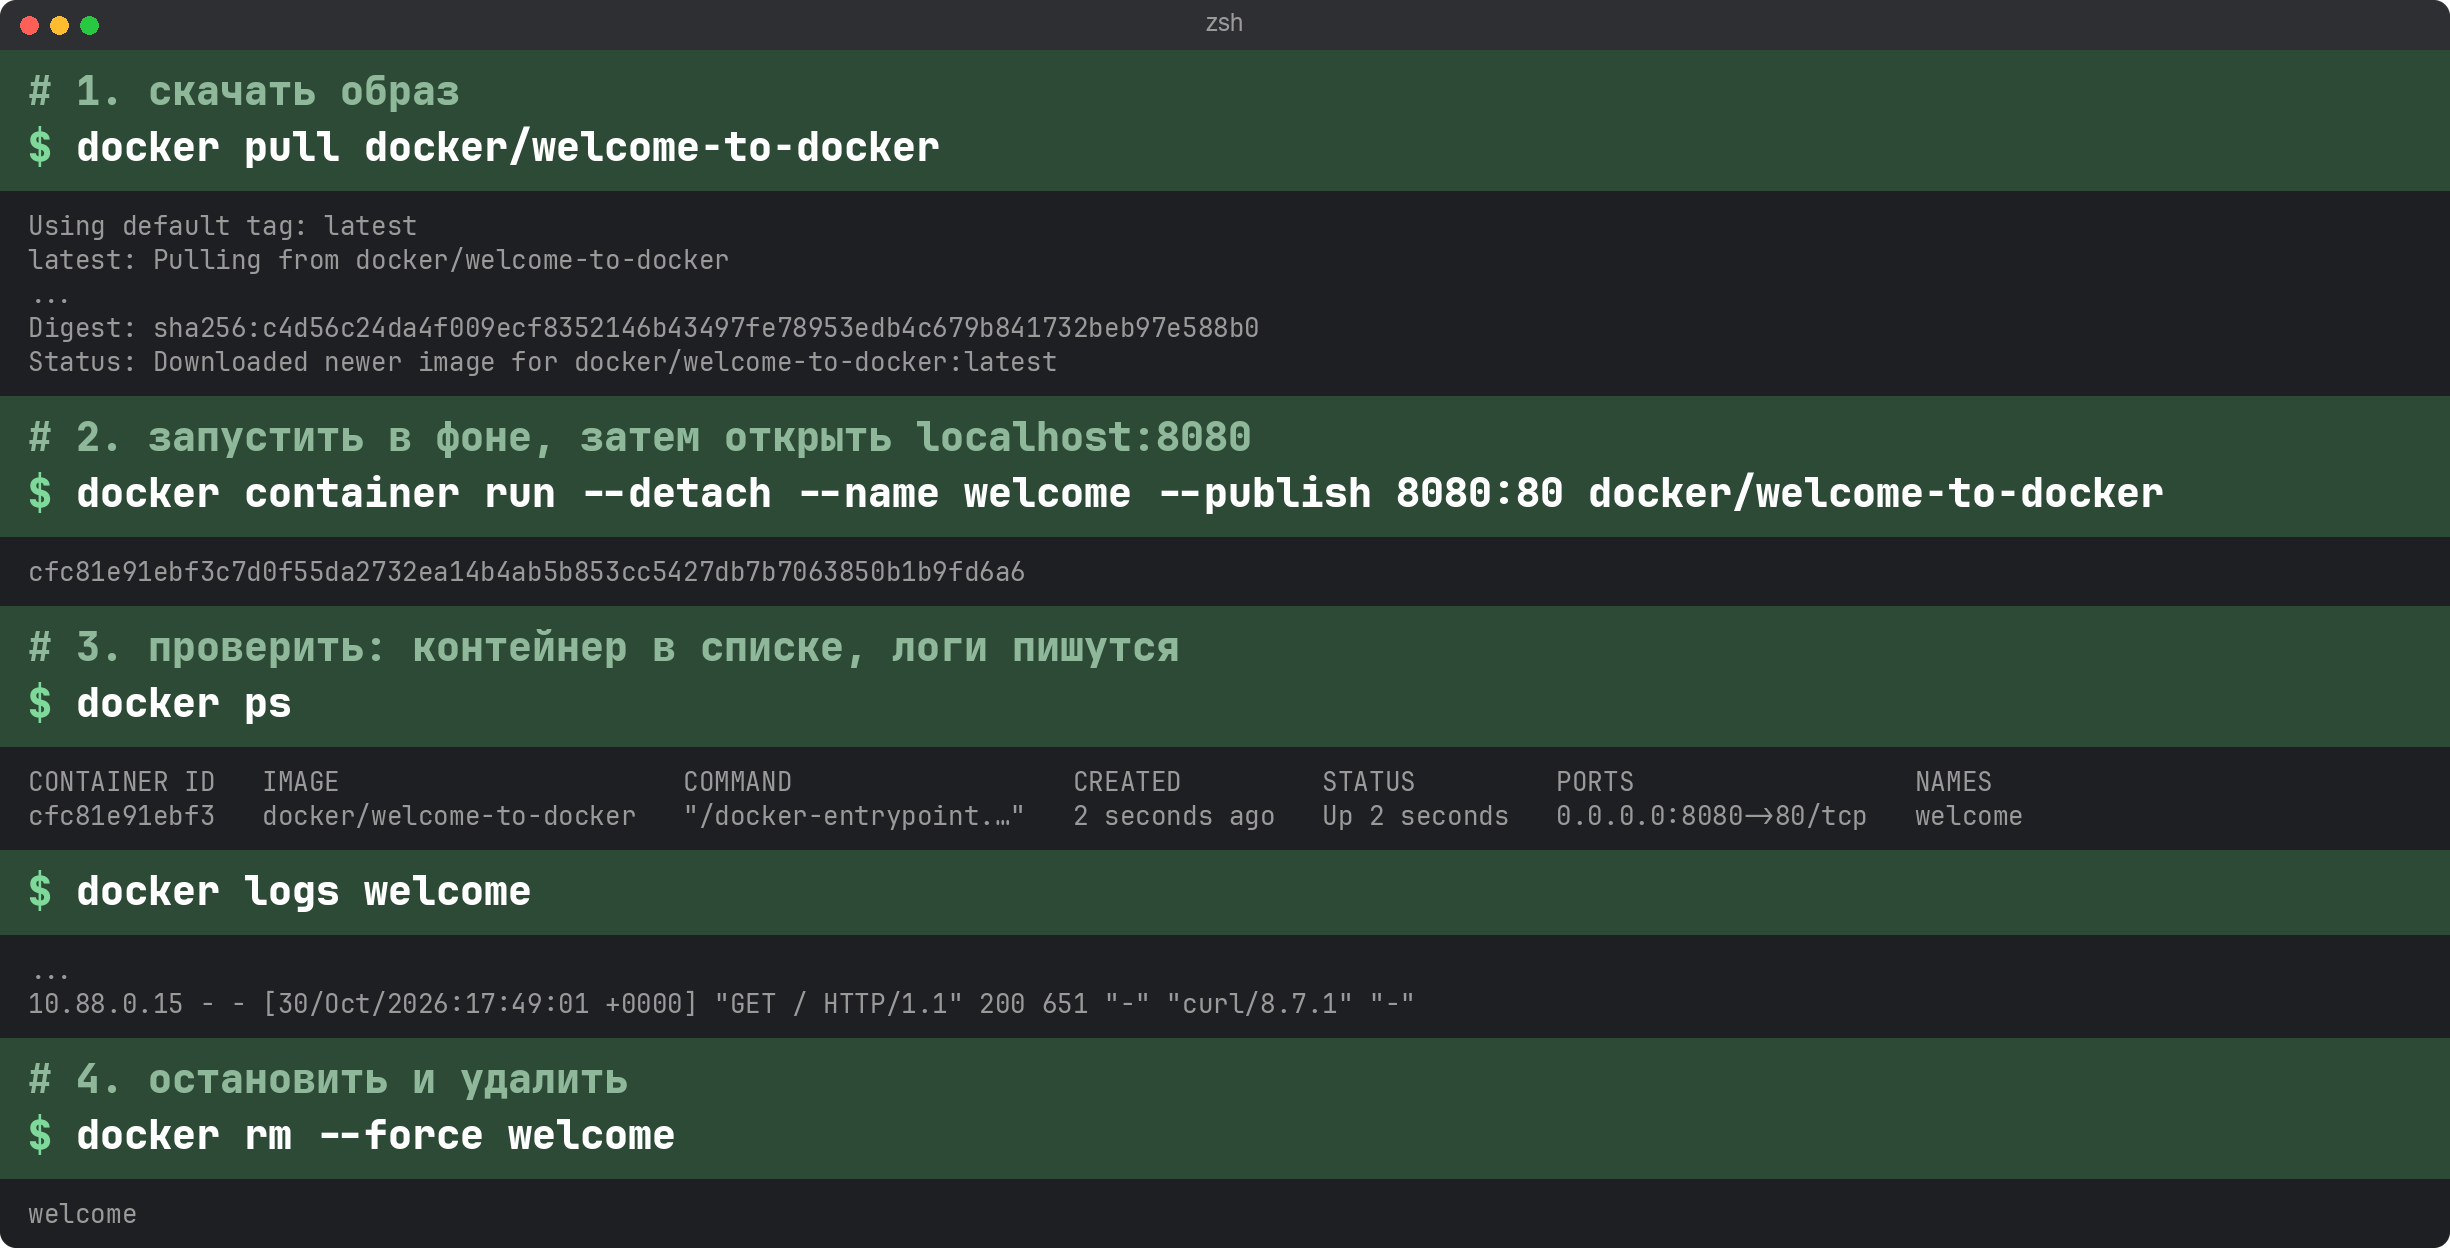
\includegraphics[width=0.78\paperwidth]{img/term/practice.png}}\par}
  \vfill
  \docs{\doclink{https://docs.docker.com/get-started/tutorials/run-an-app/}{Get started: Run an app}}
\end{frame}


\begin{frame}{Полезные ссылки}
  \footnotesize
  \begin{enumerate}
    \setlength{\itemsep}{0pt}
    \item \ulink{https://docs.docker.com/get-started/docker_cheatsheet.pdf}{Docker CLI Cheat Sheet (основа презентации)}
    \item \ulink{https://docs.docker.com/reference/cli/docker/}{Справочник Docker CLI}
    \item \ulink{https://docs.docker.com/get-started/tutorials/run-an-app/}{Get started: Run an app}
    \item \ulink{https://docs.docker.com/guides/postgresql/}{Руководство по PostgreSQL}
    \item \ulink{https://docs.docker.com/get-started/docker-overview/}{Docker overview}
    \item \ulink{https://docs.docker.com/reference/cli/dockerd/}{dockerd}
    \item \ulink{https://docs.docker.com/reference/cli/docker/image/prune/}{docker image prune}
    \item \ulink{https://docs.docker.com/reference/cli/docker/container/run/}{docker container run}
    \item \ulink{https://docs.docker.com/reference/cli/docker/system/prune/}{docker system prune}
  \end{enumerate}

\end{frame}

\end{document}
